\newpage
\section{Tomasz Leniart}

Wzory:
\begin{itemize}
    \item Równanie prostej: $ y = ax + b $
    \item Równanie parabolai $ y = ax^2 + bx + c $
    \item Równanie okręgu: $ r^2 = (x - a)^2 + (y - b)^2 $ o środku S(a,b)
\end{itemize}

\begin{table}[h]
\centering
\begin{tabular}{|c|c|c|c|c|c|c|c|c|c|c|c|}
\hline
Wykładnik Potęgi & 0 & 1 & 2 & 3 & 4  & 5  & 6  & 7   & 8   & 9   & 10   \\ \hline
Potęga 2         & 1 & 2 & 4 & 8 & 16 & 32 & 64 & 128 & 256 & 512 & 1024 \\ \hline
\end{tabular}
\caption {Potęgi 2 o wykładnikach od 0 do 10}
\end{table}

\begin{figure}[htbp]
    \centering
    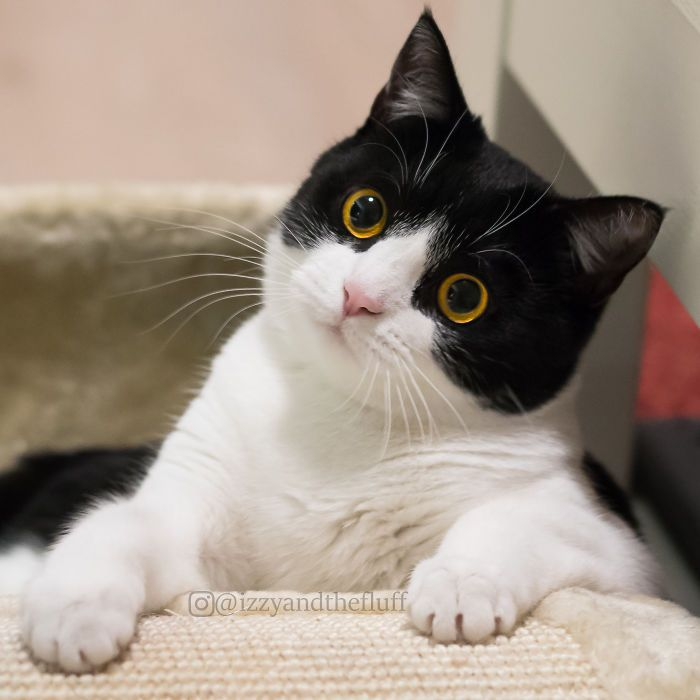
\includegraphics[scale=1.2]{pictures/image_TLeniart.jpg}
    \caption{Cute Cat Izzy - here to lift up your mood}
    \label{fig:cat}
\end{figure}

{\Large{\bf Trochę historii:}\newline}

Prezydenci USA zamordowani w czasie pełnienia urzędu:
\begin{enumerate}
    \item Abraham Lincoln (1861–1865)
    \item James Garfield (1881)
    \item William McKinley (1897–1901)
    \item John F. Kennedy (1961–1963)
\end{enumerate}

\newpage

{\Large{\bf Okręty nazawane na cześć prezydentów}\newline}

Pierwszy lotniskowiec \textit{US Navy} nazwany imieniem prezydenta Unii to „Franklin D Roosevelt” \textit{(CV 42)}. Niszczyciel typu \textit{„Arleigh Burke” DDG-80} ma za patronów wspomnianego prezydenta F.D. Roosevelta i jego małżonkę Eleanor.

Imię pierwszego prezydenta Unii – George’a Washingtona – otrzymał w dniu 9 czerwca 1959 roku \textit{SSBN-598}, pierwszy amerykański okręt podwodny o napędzie atomowym uzbrojony w pociski balistyczne. Patronem atomowego okrętu podwodnego \textit{SSBN-602} typu George Washington został 14 maja 1960 roku prezydent Abraham Lincoln. 13 lutego 1988 roku imię Lincolna nadano lotniskowcowi \textit{CVN-72} (piątej jednostce typu Nimitz).

Theodore Roosevelt został 3 października 1959 roku patronem okrętu podwodnego \textit{SSBN-600} typu George Washington. 27 października 1984 roku imię starszego Roosevelta nadano czwartemu lotniskowcowi typu \textit{Nimitz: CVN-71}. Pierwszym lotniskowcem tego typu nazwanym na cześć byłego prezydenta jest jednak \textit{CVN-69}, noszący imię Dwighta Eisenhowera.

Pierwszy prezydent Unii, który żywy doczekał wodowania lotniskowca o napędzie jądrowym nazwanego na jego cześć, to Ronald Reagan (1911–2004). Okręt nazwany imieniem Reagana to \textit{CVN-76}. Ostatni prezydent, który osobiście uczestniczył w działaniach drugiej wojny światowej na Pacyfiku, m.in. jako pilot bombowo-torpedowego Avengera na lotniskowcu „San Jacinto” – George H.W. Bush – również został za życia patronem lotniskowca: \textit{CVN-77}.

Prezydent Gerald Ford jest patronem pierwszego lotniskowca typu Gerald R. Ford (następcy lotniskowców typu \textit{Nimitz}). Drugi otrzyma nazwę John F. Kennedy. Obaj prezydenci służyli w marynarce wojennej.
